% Copyright 2004 b
% Till Tantau <tantau@users.sourceforge.net>.
%
% In principle, this file can be redistributed and/or modified under
% the terms of the GNU Public License, version 2.
%
% However, this file is supposed to be a template to be modified
% for your own needs. For this reason, if you use this file as a
% template and not specifically distribute it as part of a another
% package/program, I grant the extra permission to freely copy and
% modify this file as you see fit and even to delete this copyright
% notice. 

\documentclass{beamer}

% There are many different themes available for Beamer. A comprehensive
% list with examples is given here:
% http://deic.uab.es/~iblanes/beamer_gallery/index_by_theme.html
% You can uncomment the themes below if you would like to use a different
% one:
%\usetheme{AnnArbor}
%\usetheme{Antibes}
%\usetheme{Bergen}
%\usetheme{Berkeley}
%\usetheme{Berlin}
%\usetheme{Boadilla}
%\usetheme{boxes}
%\usetheme{CambridgeUS}
%\usetheme{Copenhagen}
%\usetheme{Darmstadt}
%\usetheme{default}
%\usetheme{Frankfurt}
%\usetheme{Goettingen}
%\usetheme{Hannover}
%\usetheme{Ilmenau}
%\usetheme{JuanLesPins}
%\usetheme{Luebeck}
\usetheme{Madrid}
%\usetheme{Malmoe}
%\usetheme{Marburg}
%\usetheme{Montpellier}
%\usetheme{PaloAlto}
%\usetheme{Pittsburgh}
%\usetheme{Rochester}
%\usetheme{Singapore}
%\usetheme{Szeged}
%\usetheme{Warsaw}


% Customize Warsaw color 
\setbeamercolor*{palette primary}{use=structure,fg=white,bg=red!50!black}
\setbeamercolor*{palette secondary}{use=structure,fg=white,bg=red!60!black}
\setbeamercolor*{palette tertiary}{use=structure,fg=white,bg=red!70!black}

% Customize Warsaw block title and background colors
\setbeamercolor{block title}{bg=red!50!black,fg=white}


% List your packages here

\usepackage[colorinlistoftodos]{todonotes}


\title[BEMOSS]{BEMOSS and Its Enhanced Applications}

% A subtitle is optional and this may be deleted
% \subtitle{Product Proposal}

\author[B.~Lauer]{Brian~Lauer\\\and
Advisor: Dr. Suruz Miah}
% - Give the names in the same order as the appear in the paper.
% - Use the \inst{?} command only if the authors have different
%   affiliation.

\institute[Bradley University] % (optional, but mostly needed)
{
  Department of Electrical and Computer Engineering\\
  Bradley University\\
  1501 W. Bradley Avenue\\
  Peoria, IL, 61625, USA
}
% - Use the \inst command only if there are several affiliations.
% - Keep it simple, no one is interested in your street address.

\date[May~31,~2019]{Friday, May~31,~2019}
% - Either use conference name or its abbreviation.
% - Not really informative to the audience, more for people (including
%   yourself) who are reading the slides online

\logo{\hfill\href{http://www.bradley.edu}{
\includegraphics[width=0.75cm]{../figs/logoBU1-Print}}}  % place logo in every page 


\subject{Mobile Robot Localization}
% This is only inserted into the PDF information catalog. Can be left
% out. 

% If you have a file called "university-logo-filename.xxx", where xxx
% is a graphic format that can be processed by latex or pdflatex,
% resp., then you can add a logo as follows:

% \pgfdeclareimage[height=0.5cm]{university-logo}{university-logo-filename}
% \logo{\pgfuseimage{university-logo}}

% Delete this, if you do not want the table of contents to pop up at
% the beginning of each subsection:
%\AtBeginSubsection[]
%{
%  \begin{frame}<beamer>{Outline}
%    \tableofcontents[currentsection,currentsubsection]
%  \end{frame}
%}
% Let's get started
\begin{document}

\begin{frame}
  \titlepage
\end{frame}

\begin{frame}{Outline}
  \tableofcontents
  % You might wish to add the option [pausesections]
\end{frame}

% Section and subsections will appear in the presentation overview
% and table of contents.
\section{Introduction}

\subsection{Overview}

\begin{frame}{Introduction}{Overview}
	\begin{itemize}
		\item \textbf{BEMOSS} or \textbf{B}uilding \textbf{E}nergy \textbf{M}anagement \textbf{O}pen \textbf{S}ource \textbf{S}oftware
		\item Virginia Tech 
		\item U.S. Department of Energy 
	\end{itemize}    
\end{frame}

%----------------------------------

\subsection{Motivation for BEMOSS} 

\begin{frame}{Introduction}{Motivation for BEMOSS}
	\begin{itemize}
		\item Track and control different loads
		\item Improve sensing and control of equipment
		\item Increase energy efficiency
		\item Encourage demand response
	\end{itemize}
\end{frame}

\subsection{Technologies Used}

\begin{frame}{Introduction}{Technologies Used}
	\begin{itemize}
		\item Communication support: Wi-Fi, Serial (RS-485), Ethernet
		\item Protocol support: BacNet, Modbus, Web, Zigbee, OpenADR, Smart Energy Profile protocols	
	
	\end{itemize}
\end{frame}


\begin{frame}{Introduction}{Technologies Used}
	\begin{itemize}
		\item Django - Python Web Framework
		\item ZeroMQ - message bus
		\item Twitter Bootstrap - front-end framework
		\item Font awesome - Icons
		\item jQuery and jQueryUI - displays data on web interface
		\item Python - language of BEMOSS
		\item VOLTTRON - Operating System
	\end{itemize}
\end{frame}

%----------------------------------

\section{Applications}

\subsection{Current Software}
\begin{frame}{Applications}{Current Software in BEMOSS}
	\begin{itemize}
		\item Lighting\_scheduler
		\item Plugload\_scheduler
		\item Illuminance based lighting control
		\item AC Fault Detection
	\end{itemize}
\end{frame}

%----------------------------------
\subsection{IoT Integration}
\begin{frame}{Applications}{IoT Integration}
	\begin{itemize}
		\item Lighting load controllers - Philips Hue
		\item Plug load controllers - WeMo Insight Switch 
		\item HVAC Controllers - Google Nest
	\end{itemize}
\end{frame}

\begin{frame}{Applications}{IoT Integration}
	\begin{figure}
		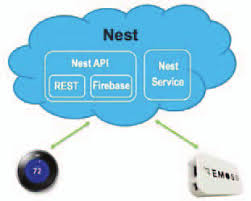
\includegraphics[scale=0.7]{../figs/nestAndBEMOSS.jpg}
	\end{figure}

\end{frame}

\begin{frame}{Applications}{IoT Integration}
	\begin{itemize}
		\item Supported devices in BEMOSS 3.5
	\end{itemize}
	\begin{figure}
		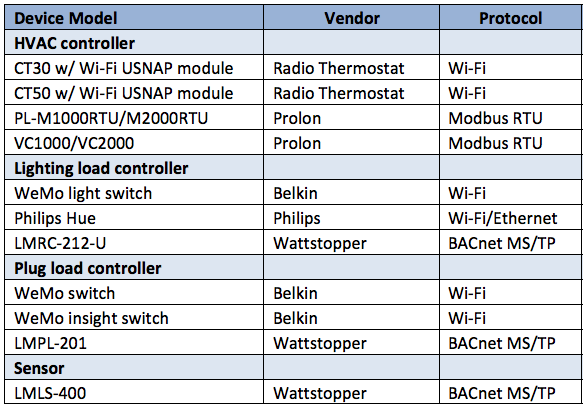
\includegraphics[scale=0.4]{../figs/bemoss35SupportedHardware.png}
	\end{figure}
\end{frame}

\subsection{Potential Applications}
\begin{frame}{Application}{Potential Applications}
	\begin{itemize}
		\item Machine learning algorithms - support vector machine, neural networks, linear regression
		\item Management of data - data filtering and distributed databases
		\item Manage multiple buildings
	\end{itemize}
\end{frame}
%----------------------------------
\section{Hardware and Software for Installation}
\begin{frame}{Hardware and Software for Installation}{}
	\begin{itemize}
		\item Laptop or desktop running Ubuntu 16.04
		\item Single-board computer - Raspberry Pi, Cubieboard, Odroid
		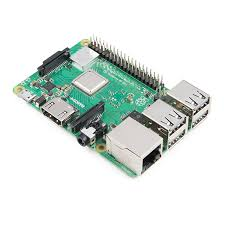
\includegraphics[scale=0.5]{../figs/rpi.jpg}
		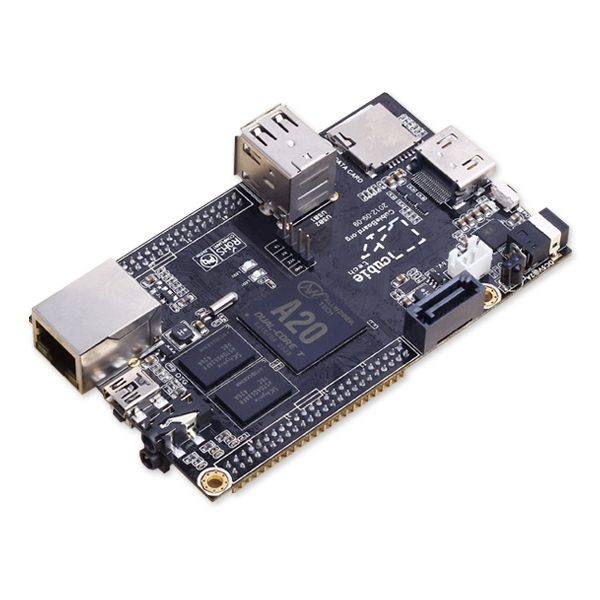
\includegraphics[scale=0.15]{../figs/cubieboard.jpg}
		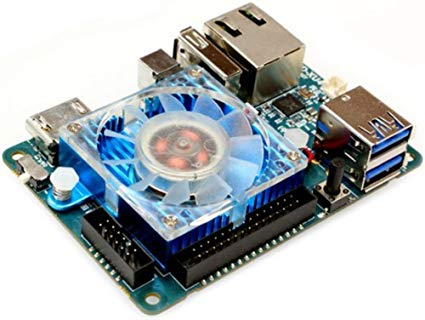
\includegraphics[scale=0.2]{../figs/odroid.jpg}
	\end{itemize}
\end{frame}

\section{Future Work}
\begin{frame}{Future Work}{}
	\begin{itemize}
		\item Machine learning algorithms
		\item Improve DC motor integration
	\end{itemize}
\end{frame}

\section*{Summary}

\begin{frame}{Summary}
  \begin{itemize}
  \item BEMOSS improves energy management in buildings
  \item BEMOSS has many applications
  \item Future work can be implemented
  \end{itemize}
\end{frame}



% All of the following is optional and typically not needed. 
%\appendix
%\section<presentation>*{\appendixname}
%\subsection<presentation>*{For Further Reading}

\begin{frame}[allowframebreaks]
  \frametitle<presentation>{References}
    
  \begin{thebibliography}{10}
    
  \beamertemplatebookbibitems
  % Start with overview books.

 
    
  \beamertemplatearticlebibitems
  % Followed by interesting articles. Keep the list short.     
   
  \bibitem{Pipattanasomporn 2015}
    M.~Pipattanasomporn.
    \newblock {\em BEMOSS: An Agent Platform to Facilitate Grid-Interactive Building Operation with IoT Devices}  	
    \newblock IEEE Power and Energy Society 2015
  \end{thebibliography}
\end{frame}

\begin{frame}
\center\Huge
Any questions?
\end{frame}
\end{document}



%%% Local Variables:
%%% mode: latex
%%% TeX-master: t
%%% End:
